\documentclass[14pt, a4paper]{extarticle}
\usepackage{GOST}
\usepackage{array}
\usepackage{verbatim}
\usepackage[detect-all]{siunitx}
\usepackage{amsmath}
\usepackage{amssymb}
\usepackage[utf8]{inputenc}
\usepackage{hyperref}
\usepackage{tempora}

\makeatletter
\renewcommand\@biblabel[1]{#1.}
\makeatother

\usepackage{listings}
\lstset{ 
	language=C,
	basicstyle=\small\sffamily, 
	numbers=left, 
	numberstyle=\tiny,
	stepnumber=1,
	numbersep=5pt,
	showspaces=false,            
	showstringspaces=false,      
	showtabs=false,             
	frame=single,            % рисовать рамку вокруг кода
	tabsize=4,      
	commentstyle=\color{green},
	keywordstyle=\color{blue}\textbf,
	numberstyle=\scriptsize\color{gray}, % the style that is used for the line-numbers
	rulecolor=\color{black},
	captionpos=t,
	breaklines=true,         % автоматически переносить строки 
	breakatwhitespace=false, % переносить строки по пробелу
	%escapeinside={\#*}{*)} 
}


\usepackage{pgfplots}
\usepackage{filecontents}
\usetikzlibrary{datavisualization}
\usetikzlibrary{datavisualization.formats.functions}

\begin{document}
	
\begin{table}[ht]
	\centering
	\begin{tabular}{|c|p{400pt}|} 
		\hline
		\begin{tabular}[c]{@{}c@{}} 
\includegraphics[scale=1]{source/b_logo.jpg} \\\end{tabular} &
		\footnotesize\begin{tabular}[c]{@{}c@{}}\textbf{Министерство~науки~и~высшего~образования~Российской~Федерации}\\\textbf{Федеральное~государственное~бюджетное~образовательное~учреждение}\\\textbf{~высшего~образования}\\\textbf{«Московский~государственный~технический~университет}\\\textbf{имени~Н.Э.~Баумана}\\\textbf{(национальный~исследовательский~университет)»}\\\textbf{(МГТУ~им.~Н.Э.~Баумана)}\\\end{tabular}  \\
		\hline
	\end{tabular}
\end{table}
\noindent\rule{\textwidth}{4pt}
\noindent\rule[14pt]{\textwidth}{1pt}
\hfill 
\noindent
\makebox{ФАКУЛЬТЕТ~}%
\makebox[\textwidth][l]{\underline{~«Информатика и системы управления»~~~~~~~~~~~~~~~~~~~~~~~~~~~~~~~~~}}%
\\
\noindent
\makebox{КАФЕДРА~}%
\makebox[\textwidth][l]{\underline{~«Программное обеспечение ЭВМ и информационные технологии»~}}%
\\

\begin{center}
	\vspace{1.5cm}
	{\bf\huge Отчёт\par}
	{\bf\Large по лабораторной работе № 4\par}
	\vspace{0.7cm}
\end{center}


\noindent
\makebox{\large{\bf Название:}~~~}
\makebox[\textwidth][l]{\large\underline{~Пять системных вызовов ОС UNIX/LINUX~}}\\

\noindent
\makebox{\large{\bf Дисциплина:}~~~}
\makebox[\textwidth][l]{\large\underline{~Операционные системы~~~~~~~~~~~~~~~~~~~~~~~~~~}}\\

\vspace{1.5cm}
\noindent
\begin{tabular}{l c c c c c}
	Студент      & ~ИУ7-55Б~               & \hspace{2.5cm} & \hspace{2cm}                 & &  Д.О. Склифасовский \\\cline{2-2}\cline{4-4} \cline{6-6} 
	\hspace{3cm} & {\footnotesize(Группа)} &                & {\footnotesize(Подпись, дата)} & & {\footnotesize(И.О. Фамилия)}
\end{tabular}

\noindent
\begin{tabular}{l c c c c}
	Преподователь & \hspace{5cm}   & \hspace{2cm}                 & & ~~~~~~Н.Ю. Рязанова~~~~~~\\\cline{3-3} \cline{5-5} 
	\hspace{3cm}  &                & {\footnotesize(Подпись, дата)} & & {\footnotesize(И.О. Фамилия)}
\end{tabular}

\vspace{0.6cm}
\begin{center}	
	\vfill
	\large \textit {Москва, 2020}
\end{center}

\thispagestyle {empty}
\pagebreak

\clearpage
\tableofcontents

\clearpage
\section*{Задание 1}
\addcontentsline{toc}{section}{Задание 1}
Написать программу, запускающую не мене двух новых процессов системным вызовом fork(). В предке вывести собственный идентификатор (функция getpid()) и  идентификаторы потомков. В процессе-потомке вывести собственный идентификатор, идентификатор предка (функция getppid()) и идентификатор группы. Убедиться, что при завершении процесса-предка потомок, который продолжает выполняться, получает идентификатор предка (PPID), равный 1 или идентификатор процесса-посредника.\par
\textbf{Код программы:}
\begin{lstlisting}[label=MultMatrVin, caption=Задание 1]
#include <stdio.h> 
#include <stdlib.h> 
#include <unistd.h>

void print_child(int child_num, char *descr)
{
	printf("child: number=%d pid=%-5d parent=%-5d group=%-5d %s\n", child_num, getpid(), getppid(), getpgrp(), descr);
}

pid_t fork_child(int child_num) 
{
	pid_t child = fork();
	if (child == -1)
	{
		perror("fork");
		exit(1);
	}
	else if (child == 0) 
	{
		print_child(child_num, "before sleep");
		sleep(2);
		print_child(child_num, "after sleep");
		exit(0);
	}
	return child;
}

int main() 
{
	pid_t child_1 = fork_child(1);
	pid_t child_2 = fork_child(2);
	
	printf("parent: pid=%-5d, child_1=%-5d, child_2=%-5d\n", getpid(), child_1, child_2);
	
	return 0;
}
\end{lstlisting}\par
\textbf{Результат работы программы:}\par
\begin{figure}[h!]
	\centering
	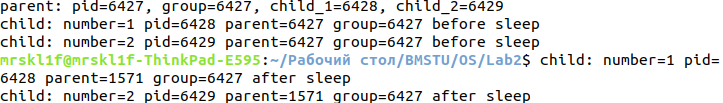
\includegraphics[width=\textwidth]{source/1.png}
	\caption{Результат работы программы}
	\label{Example1}
\end{figure}\par

\clearpage
\section{Задание 2} 
Написать программу по схеме первого задания, но в процессе-предке выполнить системный вызов wait(). Убедиться, что в этом случае идентификатор процесса потомка на 1 больше идентификатора процесса-предка.\par
\textbf{Задание 3:} написать программу, в которой процесс-потомок вызывает системный вызов exec(), а процесс-предок ждет завершения процесса-потомка. Следует создать не менее двух потомков.\par
\textbf{Задание 4:} написать программу, в которой предок и потомок обмениваются сообщением через программный канал.
\textbf{Задание 5:} в программу с программным каналом включить собственный обработчик сигнала. Использовать сигнал для изменения хода выполнения программы.
\end{document}